\documentclass{article}
\usepackage{graphicx} % Required for inserting images
\usepackage{appendix}
\usepackage{amsmath}
\usepackage[demo]{graphicx}
\usepackage{url}
\usepackage{hyperref}
\usepackage{subcaption}




\title{Advanced Analytics Project Report}

% Add your names and R-number here:
\author{Theodore Wood (R0817082), Haroon Tharwat (R0920357), \\Muath Basher (06342200), Huilin Zhang (r0964161)}


\begin{document}

\maketitle

\section{Introduction}
This report contains the assignments for the Advanced Analytics class for the Academic Year 2023-2024. Each assignment explores a unique topic discussed in the seminars. \\


\section{Assignment 1: Predictive modeling on tabular data}



\subsection{Evaluation of Dataset Processes Summary:}


\subsubsection{Data Loading \& Initial Inspection}


The dataset consists of various features related to telecom customers, including both categorical \textbf{(e.g., Gender, tariff, Handset)} and numerical data \textbf{(e.g., Age, LOS (Length of Service), Dropped Calls, average cost min)}. Additionally, there are derived features like \textbf{Peak ratio, Off Peak ratio, and ratios} involving the nature of the calls. The \textbf{Target} column indicates whether the customer churned (1) or not (0), which will be our label for predictive modeling.


\subsubsection{Data Types \& Missing Values}

Most features are numerical, but there are several categorical features: \textbf{(Gender, tariff, Handset, Usage Band, Tariff OK, and a binary representation in high-dropped calls, No Usage)}. A few columns have missing values, specifically \textbf{Dropped calls ratio, Usage Band, and call cost per min}, each with 4 missing entries.



\subsubsection{Numerical Features \& Descriptive Statistics}


The numerical features vary widely in scale and distribution. The dataset contains numerous numerical features that provide insights into customer behavior, for instance, \textbf{Age and LOS (Length of Service)} are relatively straightforward, but other features like \textbf{Peak calls Sum, Peak mins Sum, and average cost min} could have more complex distributions and relationships with the target variable. The presence of skewness in some of these features suggests variability in customer usage patterns and behaviors.
 There are also features that seem to be ratios or calculated metrics, such as \textbf{Peak ratio, Off Peak ratio, and Nat-InterNat Ratio}.




\subsubsection{Outlier Detection}


The IQR method confirmed the presence of outliers in key features potentially related to churn, such as \textbf{Dropped Calls (926 outliers), Peak calls Sum (215 outliers), and average cost min (310 outliers)....}. These features are critical in understanding customer behavior related to churn. These outliers could either represent true extremes in customer behavior or data entry errors. We will evaluate the relevance of outliers in the context of churn prediction. In cases where outliers represent extreme but valid customer behaviors, they might be crucial for our predictive model.



\subsubsection{Target Variable Analysis}


 The target variable, target, accurately reflects customer churn without missing values. The class distribution indicates an imbalance - shows notable positive skewness - with approximately \textbf{14.77\%} of customers having churned. This imbalance is critical for model evaluation and selection, suggesting the need for strategies such as weighted classes in models, oversampling of the minority class, or specialized metrics that account for imbalance.




\subsubsection{Additional Insights}
 
\begin{itemize}
    \item The dataset contains a unique identifier Id for each customer, which should be excluded from model training to prevent overfitting.
    \item Features like Gender, tariff, and Handset are categorical and will need encoding. 
    \item Call-related features and costs are likely significant indicators of churn, necessitating detailed analysis and potential feature engineering to capture customer behavior effectively.
    \item The presence of a No Usage feature could be a strong indicator of churn, highlighting customers who may have already disengaged from the service.
\end{itemize}


\subsection{Data Visulazations:}

\subsubsection{Distribution of Key Numerical Features}

\begin{itemize}
    \item \textbf{Age} : The age distribution is fairly normal but slightly right-skewed, indicating a younger customer base with fewer older customers. This skew suggests that retention strategies might need to be tailored differently across age groups, with a focus on the preferences of a younger demographic.

\item \textbf{Length of Service (LOS) }: The LOS feature demonstrates a uniform distribution among the dataset, suggesting that the customer base consists of a balanced mix of new and tenured subscribers.

\item \textbf{Dropped Calls }: The distribution of dropped calls is highly right-skewed, with most customers experiencing few dropped calls. However, a small subset of customers encounters a higher number of dropped calls, which could be a significant factor in churn.

\item \textbf{Total Cost }: Similar to dropped calls, total cost also shows a right-skewed distribution. While most customers incur lower costs, there is a notable presence of customers with higher charges, which may contribute to dissatisfaction and increased churn risk.
\end{itemize}


\begin{figure}[h]
\centering
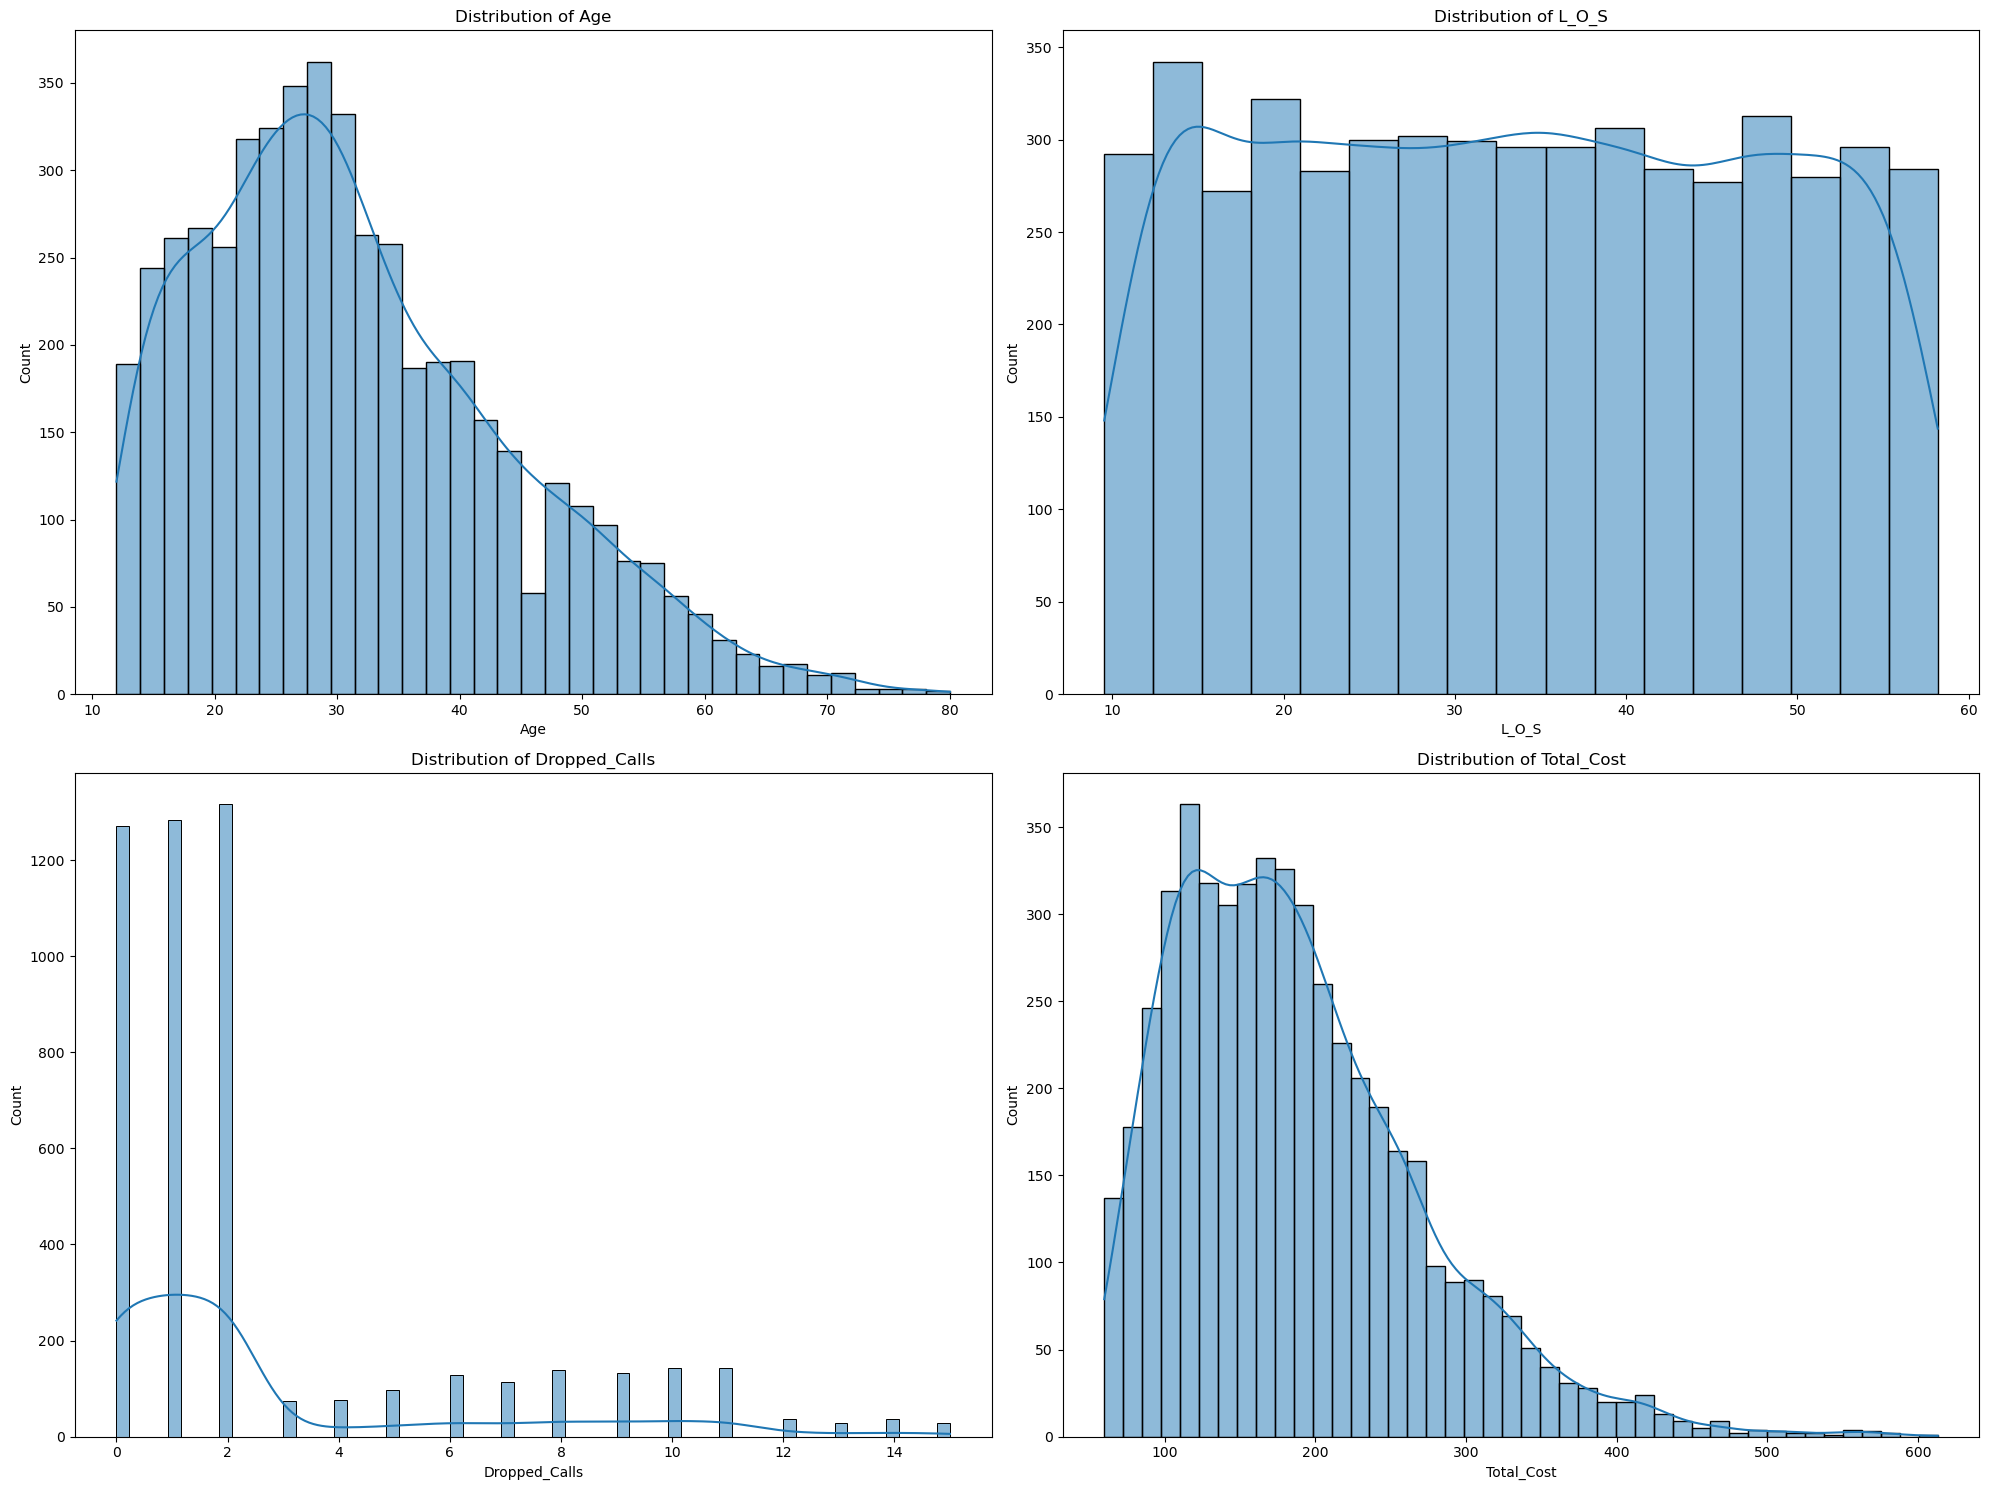
\includegraphics[width=0.8\linewidth]{Distribution of Key Numerical Features.png}
\caption{Distribution of Key Numerical Features}
\label{fig:distribution}
\end{figure}


\subsubsection{Categorical Features Analysis}

\begin{itemize}
    \item \textbf{Gender}: Churn does not appear to significantly differ by gender, suggesting that male and female customers are equally likely to churn.

    \item \textbf{Tariff Plans}: Distinct patterns emerge when analyzing churn by tariff plans. Some plans, such as CAT 200, exhibit a higher proportion of churn, which may indicate issues with plan pricing or features.

    \item \textbf{Handset Types}: Handset type seems to play a role in churn, with specific models showing different churn rates. This could imply that customer satisfaction with their devices influences their decision to stay with the provider.
\end{itemize}


\begin{figure}[h]
\centering
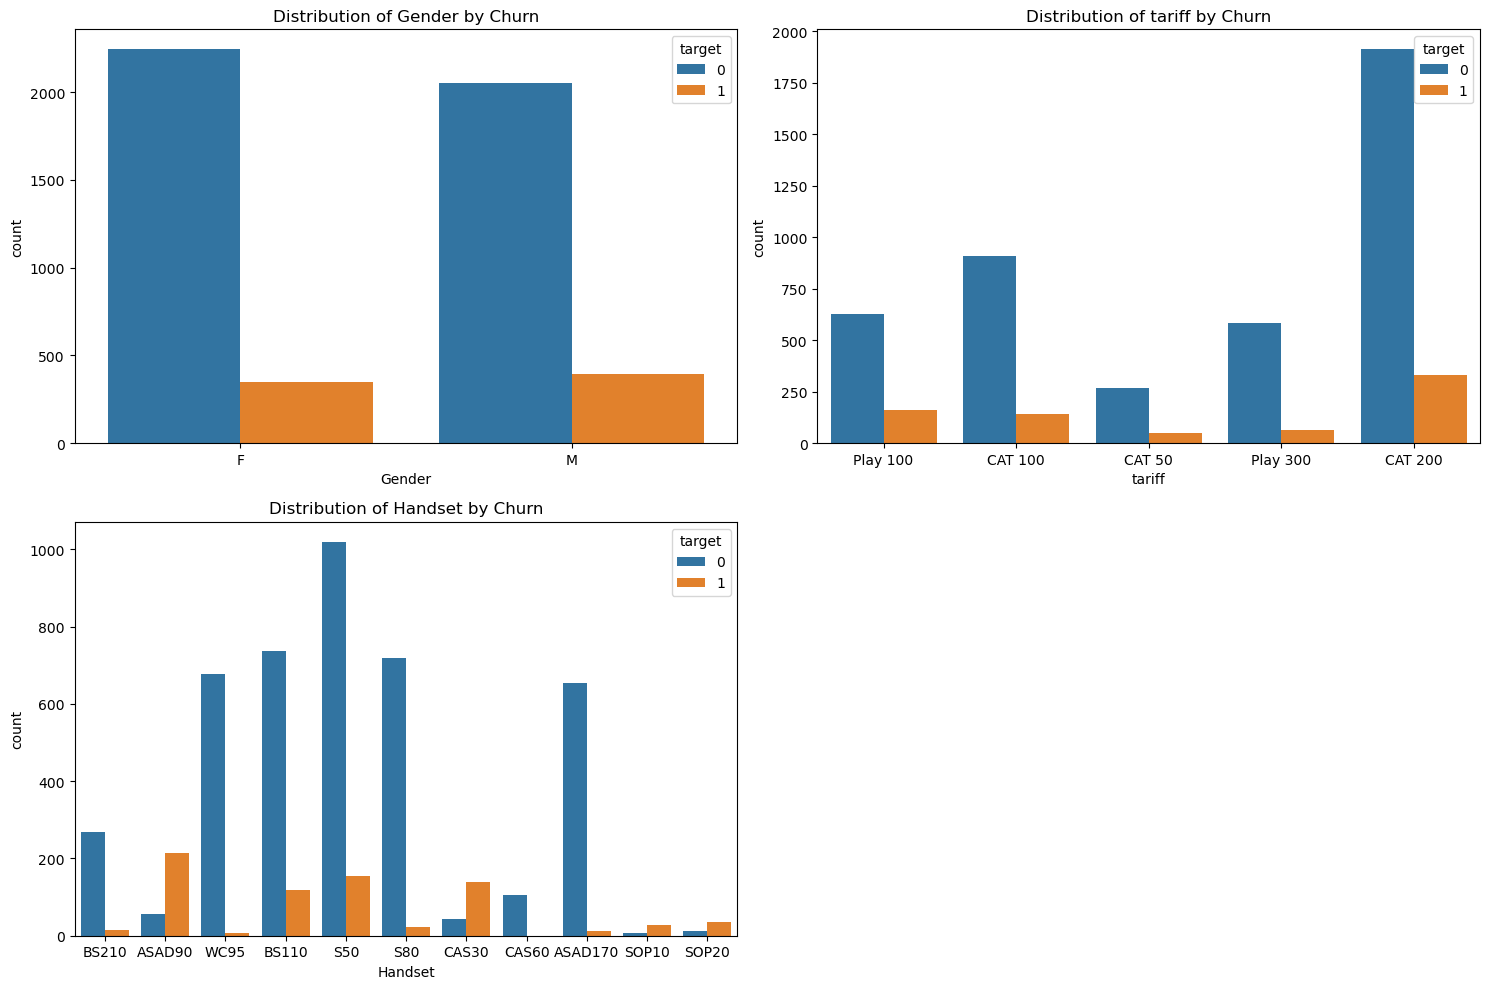
\includegraphics[width=0.8\linewidth]{Categorical Features Analysis.png}
\caption{Categorical Features Analysis}
\label{fig:distribution}
\end{figure}











\subsubsection{Correlation Matrix of Numerical Features and Target Variable}


The correlation matrix indicates that most numerical features have a relatively low correlation with the target churn variable. However, Dropped Calls has a mild positive correlation with churn, which aligns with the distribution findings and suggests that service quality is an area of concern affecting customer retention.

\begin{figure}[h]
\centering
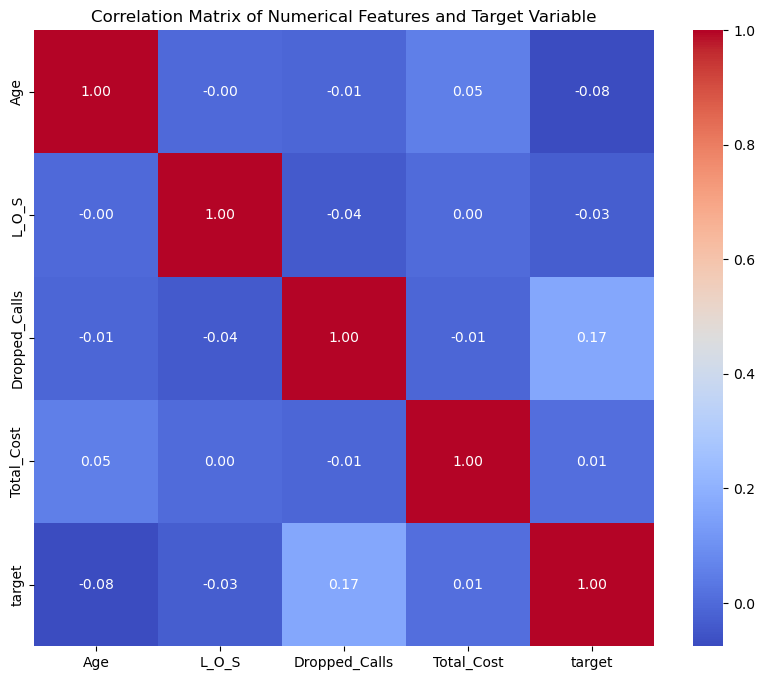
\includegraphics[width=0.3\linewidth]{Correlation Matrix of Numerical Features and Target Variable.png}
\caption{Correlation Matrix of Numerical Features and Target Variable}
\label{fig:distribution}
\end{figure}


\subsubsection{Relationship between Total Cost and Dropped Calls}

The scatter plot displays a relatively discrete pattern, with most data points clustered at lower values of dropped calls. This pattern suggests that for most customers, the total cost does not significantly increase with the number of dropped calls. There does not appear to be a strong linear relationship, as the points do not form a clear ascending or descending trend that would suggest a direct correlation. However, there is a visible range of total costs across all levels of dropped calls, which indicates variability in the cost that is not explained solely by the number of dropped calls.

The lack of a strong relationship here implies that the total cost a customer incurs might be influenced by a combination of factors beyond just the number of dropped calls. This suggests that a more complex model may be necessary to predict total costs accurately, taking into account multiple variables simultaneously.

\begin{figure}[h]
\centering
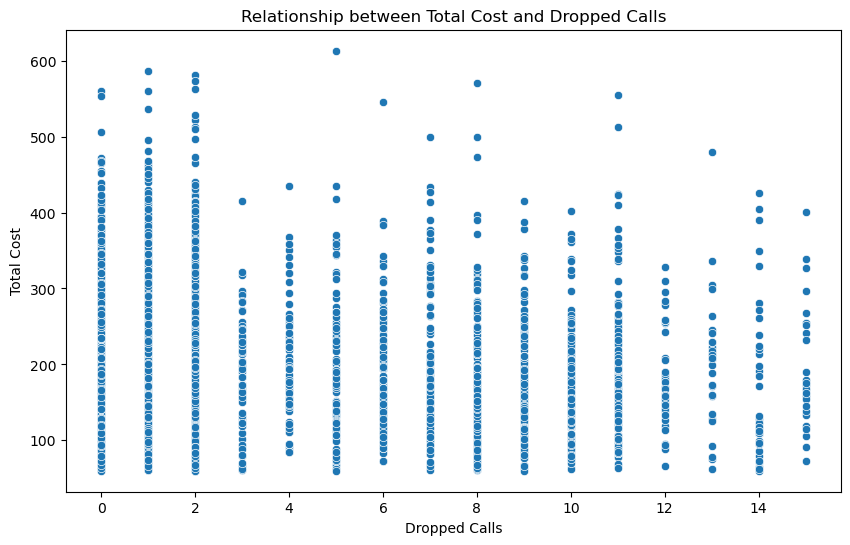
\includegraphics[width=0.4\linewidth]{Relationship between Total Cost and Dropped Calls.png}
\caption{Relationship between Total Cost and Dropped Calls}
\label{fig:distribution}
\end{figure}


\subsubsection{Relationship between Age and Length of Service}

The scatter plot for age and length of service displays a wide spread of data points with no discernible pattern or trend, indicating that there is no strong linear relationship between a customer's age and their length of service. The data points are distributed across all ages and service lengths, suggesting that the telco's customer base is varied and that customer tenure does not necessarily increase with age. This could imply that the telco is equally retaining younger and older customers, or it could suggest that age is not a determinant factor in how long customers stay with the provider.

The absence of a trend between age and length of service suggests that other factors might play a more significant role in determining customer tenure. For instance, customer satisfaction, service quality, and pricing might be more relevant factors.

\begin{figure}[h]
\centering
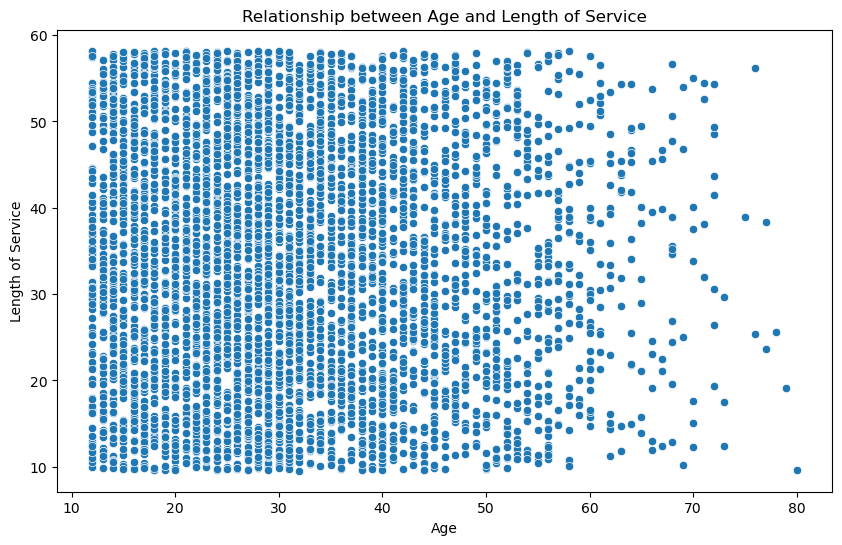
\includegraphics[width=0.4\linewidth]{Relationship between Age and Length of Service.png}
\caption{Relationship between Age and Length of Service}
\label{fig:distribution}
\end{figure}




\subsubsection{Key Findings and Additional Insights}

\begin{itemize}
\item \textbf{Service Quality Improvement}: Given the skewness in dropped calls and its correlation with churn, enhancing network quality and reducing call drops should be a priority.
\item \textbf{Tariff Plan Optimization}: The variation in churn rates across tariff plans calls for a review of plan features and pricing structures to better meet customer needs and improve retention.
\item \textbf{Device Satisfaction}: The differences in churn by handset type suggest that customers' hardware experiences significantly influence their likelihood to churn. Efforts to improve device offerings or support could mitigate churn.

\end{itemize}




\subsection{Encoding Categorical Variables:}

\textbf{Variables for Encoding}
\begin{itemize}
    \item \textbf{Gender}: gender is binary and can be label-encoded.


 \item \textbf{Connect Date}: feature engineering is implemented to extract useful information like tenure, month, or year, which can be more directly related to churn prediction.

 \item \textbf{Tariff}: nominal without an inherent order. Different tariff plans would best be one-hot encoded to capture their impact on churn without implying any hierarchy.


     \item \textbf{Handset}: nominal, representing different models or types of handsets ( 11 types).


     \item \textbf{Usage Band}: \textbf{'Med', 'MedLow', 'MedHigh', 'High', 'Low'}, it indicates an inherent order among the categories, which suggests that label encoding would be appropriate for this variable. Label encoding can capture the ordinal relationship between these categories, which could be informative for the model.

    
\item \textbf{Tariff OK}: unique categories in 'Tariff OK' are \textbf{'OK', 'High CAT 100', 'High CAT 50', 'High Play 100'}, this variable might be better suited for one-hot encoding given the nominal nature of these categories, where there's no inherent order and each represents a distinct group

\item \textbf{High Dropped Calls}: binary,  label-encoded.

\item \textbf{No Usage}: binary (indicating whether a customer has used the service), it is label-encoded.

\item \textbf{ID}: This is a unique identifier for each customer. It should not be encoded but rather dropped from the feature set used for modeling, as it doesn't provide predictive value for churn.


\end{itemize}


\subsection{Outlier Treatment \& Scaling Numerical Features}

\textbf{Outliers}: Age: 67, LOS: 0, Dropped Calls: 926, Total Cost: 111

\begin{itemize}
    \item \textbf{Age}: is not heavily skewed, so extreme values might be errors or rare genuine cases. If they're reasonable (e.g., within a possible age range for customers), they can be kept. Otherwise, capping or removing extreme ages that don't make sense (e.g., age > 100) might be warranted.
    
\item \textbf{LOS (Length of Service)} : No treatment is necessary since there are no outliers.

\item \textbf{Dropped Calls}: since this variable has a significant number of outliers and dropped calls can impact customer churn, we considered a log transformation to reduce skewness without losing information on the genuine high values. The outliers decreased from 962 to 28.

\item \textbf{Total Cost}: given the nature of cost-related data and given the spread and the number of outliers, a Box-Cox transformation is appropriate because it can handle and adjust various degrees of skewness more effectively than a simple log transformation. The outliers were reduced from 111 to 4.

\end{itemize}


\begin{figure}[h]
\centering
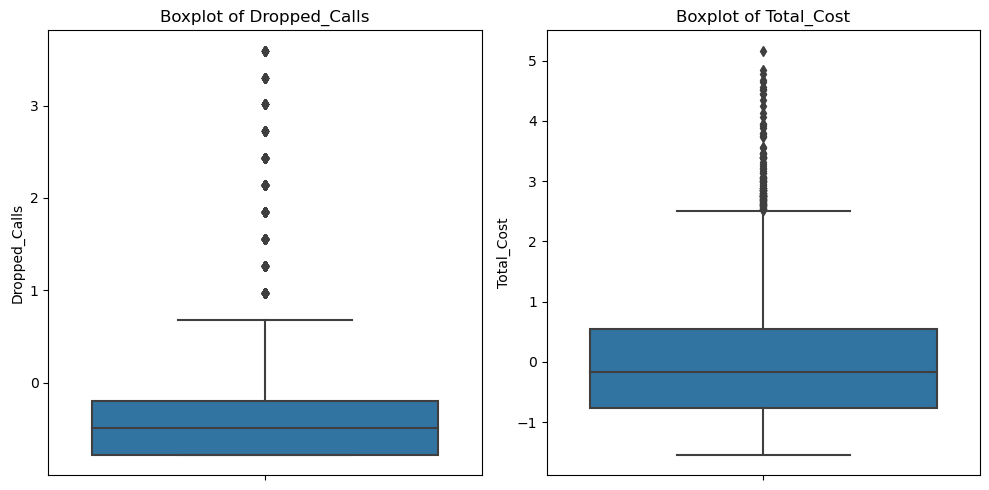
\includegraphics[width=0.3\linewidth]{Significantly skewed features.png}
\caption{Significantly skewed features}
\label{fig:distribution}
\end{figure}



\subsection{Enhanced Interaction Terms Creation}
We introduced interaction terms into our predictive model to capture the combined effects of two features that are not evident when these features are considered independently. By exploring these interactions, we can potentially unveil complex dependencies that could improve the model's accuracy and explanatory power.


The interaction terms were generated by multiplying two relevant features together, thus creating a new feature that represents their joint effect on the response variable. This approach was systematically applied to selected pairs of features based on domain knowledge and preliminary data analysis indicating potential interactions.

The following pairs of features were identified for interaction term creation:
\begin{itemize}
    \item Total Cost and Length of Service (LOS)


\item Total Cost and Dropped Calls
\item Length of Service (LOS) and Dropped Calls
\item Average Peak Usage (Ave Peak) and Total Cost
\item Sum of Peak Calls and Sum of OffPeak Calls
\item International Minutes Sum and Total Cost
\item Dropped Calls and Call Cost per Minute
\item National Calls and International Minutes Sum
\end{itemize}


The same interaction terms created in the training dataset were also computed in the test dataset using the identical methodology to ensure consistency in model application. 



\subsection{Defining the Transformations}
Transformations in data preprocessing play a crucial role in aligning the raw data with the requirements of machine learning models. In our project, transformations involved handling missing values, encoding categorical features, normalizing numerical data, and engineering new interaction terms. Specifically, KNN imputation was utilized for numerical columns to estimate missing values based on the nearest neighbors, which helps in preserving the inherent structure of the data. Categorical columns were imputed with the most frequent category to avoid any bias that might arise from other imputation techniques.

\subsection{Setting Up the Model}
The models were set up as part of a machine learning pipeline, ensuring a systematic flow of data from preprocessing to the final prediction. The pipeline was constructed using scikit-learn and imblearn libraries, which included steps for data preprocessing (e.g., scaling and encoding), handling class imbalance using SMOTE, and finally the classification models. The classifiers included Random Forest, Gradient Boosting, XGBoost, Logistic Regression, and SVM. Each model was equipped to handle the specifics of the input data while being capable of producing probability outputs needed for ROC curve analysis.

\subsection{Model Pipeline}
The model pipeline integrated several preprocessing steps with the actual machine learning algorithm. This integration facilitates the seamless transformation of data followed by the training process, without the need for repetitive manual intervention. The pipeline approach not only simplifies the code but also helps in avoiding common mistakes like data leakage between training and testing phases.

\subsection{Performance of several models on training data}

In the ROC Curves for Various Models figure below, each line on the graph represents a different model, with the area under the curve (AUC) providing a quantitative measure of each model's performance.


\begin{figure}[h]
\centering
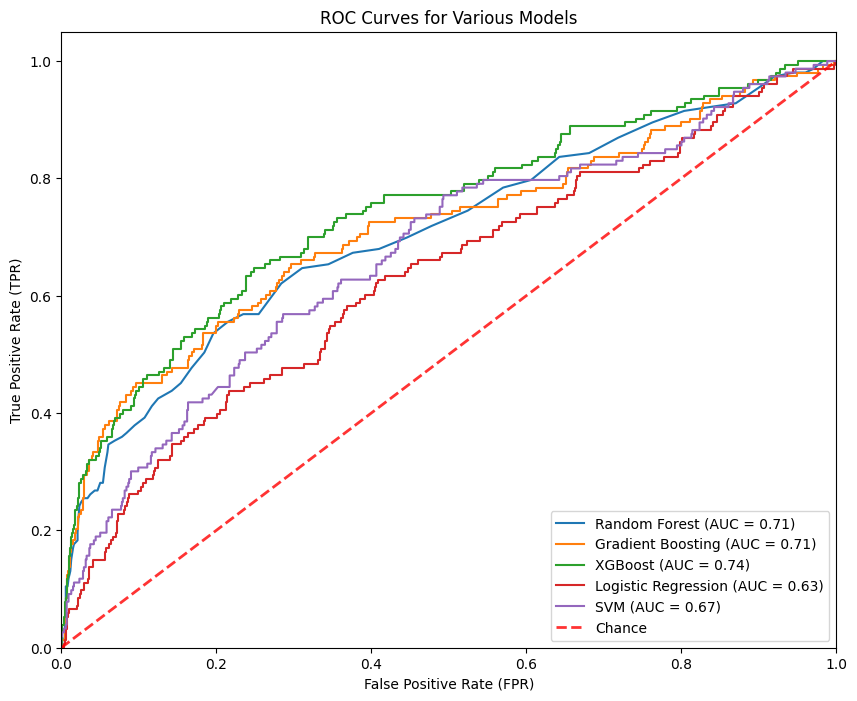
\includegraphics[width=0.5\linewidth]{models.png}
\caption{ROC Curves for Various Models}
\label{fig:distribution}
\end{figure}


\textbf{Explanation of the Results:}
\begin{itemize}
    \item Random Forest \& Gradient Boosting: Both models have an AUC of 0.71, indicating a good predictive performance, better than a random guess but with room for improvement. The similar performance suggests that both models, which rely on decision trees, are equally effective for the data and settings used.
    \item XGBoost: This model shows a slightly better performance with an AUC of 0.74, making it the most effective among the tested models at distinguishing between the classes. XGBoost often performs well on a variety of tasks due to its robust handling of various data types and its gradient boosting framework that reduces overfitting.
    
    \item Logistic Regression: With an AUC of 0.63, this model performs less effectively compared to the ensemble methods. Logistic regression is a simpler model and might be underfitting the dataset or not capturing complex patterns as effectively as the tree-based models.
    \item SVM (Support Vector Machine): This model has an AUC of 0.67, indicating a fair performance that is better than logistic regression but not as good as the tree-based methods. SVMs are effective in high-dimensional spaces or when the classes are well separable but might require careful tuning of parameters such as the kernel type.

    
    
\end{itemize}




Curve Proximity to Top-Left Corner,the closer the curve follows the left-hand border and then the top border of the ROC space, the more effective the model. XGBoost comes closest to the top-left corner, indicating its superior performance on this dataset.



\subsection{Test Dataset Preprocessing}
The test dataset underwent a similar preprocessing pipeline as the training set to maintain consistency. This includes the same imputation strategies, outlier handling, skewness adjustments, and encoding of categorical variables. Ensuring that both training and test data follow the same preprocessing steps is crucial for the reliability of the model predictions.



\subsection{ Distribution of Predicted Probabilities on Test Data}

The histogram of predicted probabilities shows the frequency distribution of predicted probabilities for churn across all predictions made by the model. This plot provides insights into how confidently the model is making predictions and the general skew of these probabilities.
\begin{itemize}


    

\item  \textbf{Shape and Trends}: The distribution is skewed towards lower probabilities with a peak around 0.1-0.2, suggesting that the model predicts a lower likelihood of churn for a majority of the cases.
\item  \textbf{Interpretation}: The density of predictions on the lower end of the probability scale indicates that the model finds most of the customers less likely to churn, with fewer customers showing higher churn probabilities. This could either reflect the true distribution of churn within the dataset or indicate a model that is conservative about predicting churn.
\end{itemize}



\begin{figure}[h]
\centering
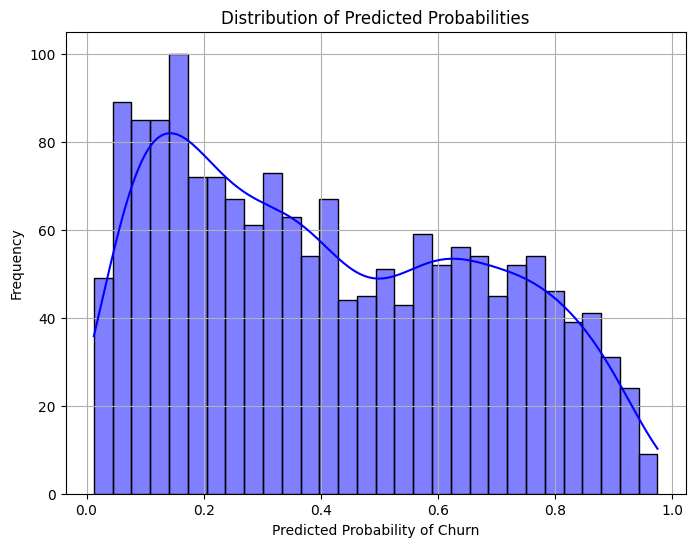
\includegraphics[width=0.4\linewidth]{ass.png}
\caption{Distribution of Predicted Probabilities}
\label{fig:distribution}
\end{figure}

\begin{figure}[h]
\centering
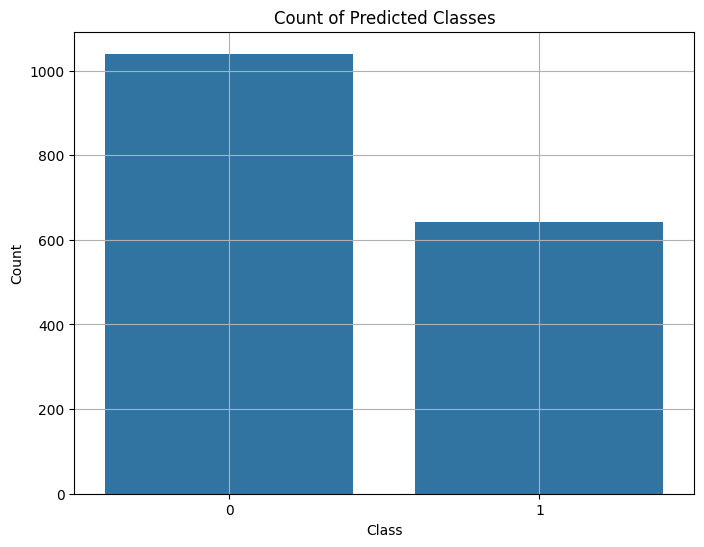
\includegraphics[width=0.4\linewidth]{count of preit.png}
\caption{Predicted Probability of Churn}
\label{fig:distribution}
\end{figure}


\subsection{ Count of Predicted Classes}
The count plot and accompanying data display the total counts of classified results (0 for 'No Churn' and 1 for 'Churn') based on a chosen threshold 0.5.

\begin{center}
\begin{tabular}{|c|c|}
\hline
\textbf{Class} & \textbf{Count} \\
\hline
0 & 1040 \\
\hline
1 & 642 \\
\hline
\end{tabular}
\end{center}

\subsection{ Critical Review}

Our methodology provides a foundation to critically review the evaluation metrics chosen by management, namely the profit @ top-20, and how it aligns with the AUC.


\textbf{Profit @ Top-20}
\begin{itemize}

    \item This metric concentrates on the most likely churners that can impact profitability, emphasizing the practical business impact of the model. From the analysis, this seems particularly pertinent as it aligns with the business's focus on actionable insights from a limited subset of high-value predictions. However, there are several points to consider:

    \item  Precision vs. Recall Trade-Off: the models, particularly the XGBoost with the highest AUC of 0.74, demonstrate a good ability to distinguish between churners and non-churners across all thresholds. However, profit @ top-20 inherently values precision over recall, emphasizing correct predictions within a small segment of high-risk customers. This might lead to overlooking other potential churners who fall just outside the top 20 but still represent significant profitability risks.
    
    \item Resource Allocation: By focusing on top-20 churn predictions, the company can optimize resource allocation (e.g., targeted offers or customer engagement strategies), but this may neglect a broader strategy that includes moderately risky customers, potentially increasing overall churn.

\end{itemize}
\textbf{AUC (Area Under the Curve)}
AUC measures the model's ability to rank customers by their likelihood of churning, irrespective of any specific classification threshold. This metric provides a comprehensive view of model performance across all possible classification thresholds, ensuring the model's general effectiveness. The findings suggest that \textbf{General Model Effectiveness:} With AUC values for different models ranging from 0.63 to 0.74, there's a clear indication that your models can generally distinguish between churners and non-churners. However, the AUC does not focus on the "profitability" of correctly predicting top churners, which is critical from a business perspective.
   
\textbf{Alignment of Metrics and Business Objectives}:
Considering the focus of the business on limiting intervention costs, the profit @ top-20 is a strategically chosen metric. It ensures that the business's limited resources are directed towards the customers most likely to churn and whose retention would contribute most to the company's profitability. However, this metric might lead to potentially high-value customers being neglected if they are not ranked in the top 20. This could be mitigated by:
\begin{itemize}
 \item Integrating Customer Lifetime Value (CLV): Adjusting the profit @ top-20 to consider not only the immediate profitability but also the long-term value that could be lost if a high-value customer churns.
 \item Balanced Metric Approach: Combining AUC with profit @ top-20 could provide a more holistic view of model performance, ensuring broad effectiveness while also maximizing impact on profitability.
\end{itemize}

\textbf{Alternative Metrics to discover }:
\begin{itemize}
\item Precision at k: Could be adapted to focus on the top-20 predictions, ensuring that the model is evaluated based on its accuracy at the top of the list, which is directly relevant to the profit @ top-20 metric.
\item Cost-sensitive accuracy: Incorporating the costs or profits associated with correct or incorrect predictions would allow the model's performance to be evaluated in terms that directly reflect business outcomes.
\end{itemize}

The choice of profit @ top-20, while strategically sound for focusing efforts and resources, may benefit from a broader perspective brought by integrating AUC and other relevant metrics like CLV to provide a more comprehensive assessment of the model's impact on business objectives. This approach will ensure that while the model is optimized for immediate profitability, it also supports long-term customer retention strategies.








\section{Image Classification}

For this assignment, we approached the multilabel classification model, where we attempt to formulate and train a model that can predict the top 20 most frequent tags that appear in the dataset of the games. \\

Our approach for creating this model was to first reduce the file size of the images by downscaling them to half-size while retaining the file type extension. Then, we created a new dataset with our \verb|preprocess_images()| function, which returned an array with the images, the game title, and the game tags. Our train-test split utilized scikit-learn's \verb|train_test_split()| function, which we then used to compute the top 20 most common tags by iterating over both the newly created train set and test set as one single file. 

First, we created a python script that reduced the size of the images in the image folder by half (but keeps the file type the same), so that when we reevaluate the model we do not need to store the 40GB folder on the hard drive. 
\\
For the actual implementation of the model, we used the keras framework, which is a high-level API of tensorflow. From the JSON file, we extract each game's title, tags, and screenshots into a pandas dataframe. We also preprocessed the images so that they all were formatted in the same shape (224,224,3). Some of the images were corrupted or irretrievable, so we also added a script that would notify us of such an event, and would ignore that file. Additionally, some images would not be correctly formatted into the desired (224,224,3) shape, so we also implemented a script that would ensure they would not be added to the final dataset, and would notify us of this. \\

We limited the dataset to only include tags that belonged to the top 20 most common tags. To create a training and test dataset, we utilized scikit-learn's built-in \verb|train_test_split()| function, and then proceeded with the construction of the model. This split is done at the level of the game, so each image belonging to a game is placed in either the train set or test set. Our specific implementation created the train test split first, and then retrieved only the 20 most frequent tags amongst both the train data and test data. We applied a one-hot encoding for each game image, which were used as labels for our model. This means that every image had a 0 (not present) or 1 (present) for each label (tag). \\

Due to the problem complexity, we added several layers to our sequential CNN model, including 4 'relu' activation layers. The sequential model was built as follows:
\begin{verbatim}
    model = tf.keras.Sequential([
    keras.Input(shape=(224,224,3)),
    tf.keras.layers.Conv2D(32, (3, 3), activation='relu',
    tf.keras.layers.MaxPooling2D((2, 2)),
    tf.keras.layers.Conv2D(64, (3, 3), activation='relu'),
    tf.keras.layers.MaxPooling2D((2, 2)),
    tf.keras.layers.Conv2D(128, (3, 3), activation='relu'),
    tf.keras.layers.MaxPooling2D((2, 2)),
    tf.keras.layers.Flatten(),
    tf.keras.layers.Dense(128, activation='relu'),
    tf.keras.layers.Dropout(0.5),
    # Output layer with 20 neurons for multilabel classification
    tf.keras.layers.Dense(20, activation='sigmoid'])  
\end{verbatim}

\begin{figure}[h!]
    \centering
    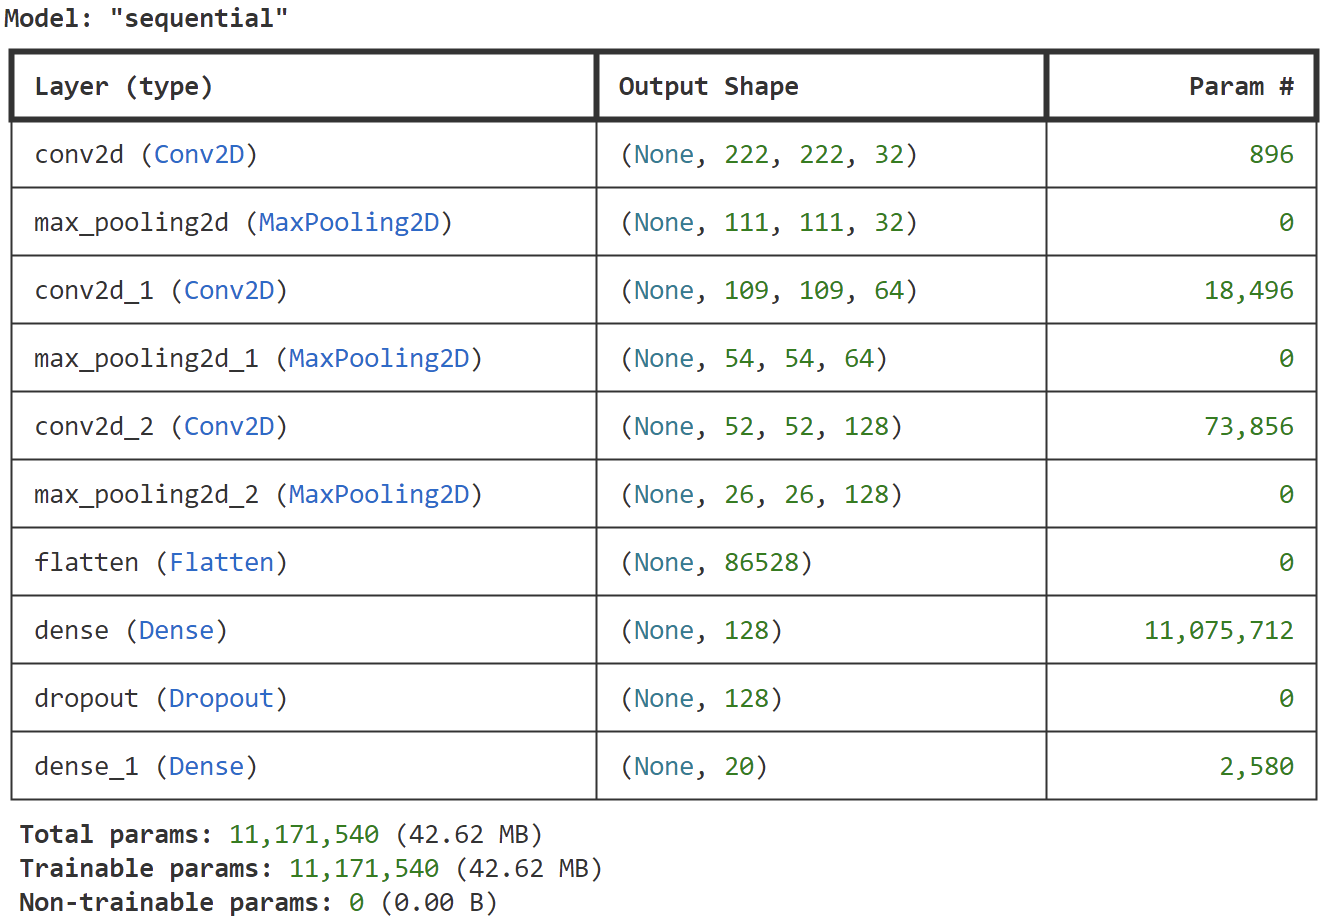
\includegraphics[width=0.8\linewidth]{Screenshot 2024-05-25 230030.png}
    \caption{Sequential Model Layers}
    \label{fig:enter-label}
\end{figure}

The total parameters of the model come to 11,171,540. The first layer is an input layer to intake the raw information of the images. The next layer is a convolutional layer with a rectified linear unit (ReLu) activation function. This allows the model to extract features from the input. We start with a depth of 32 on the first convolutional layer, then 64, and finally 128 for the last convolutional layer. \\

The maxpooling layer is implemented to reduce dimensionality while retaining the most important features extracted from the previous layers. These maxpooling layers are applied after every convolutional layer. The flattening layer is applied so that the information is presented in a shape that the next layer, the Dense layer, can process it. The Dense layer functions so that all neurons are interconnected, and this is where classification occurs. The Dropout layer is intended as a precaution to reduce overfitting by randomly selecting a number of features to be set to zero during training. The final layer is a Dense layer with a sigmoid activation function. This is how we determine the probabilities of whether a label applies to a given image. \\
For storing the data, we rounded these probabilities to the nearest integer (0 or 1), which we can use to compare with the actual labels. These probabilities are then stored in a csv file, \verb|binary_predictions.csv|. We can also compare the predicted results with the actual results in the file \verb|y_test.csv|.\\

Again, due to the high complexity of the model, as well as the format of the input data (images), the computation time required to train the model is high. Each epoch took over 20 minutes to compute, but we found that increasing the number of epochs further only hindered performance on the test set. Thus, we only iterate over the entire training set 3 times, using batch sizes of 64. \\

\begin{figure}
    \centering
    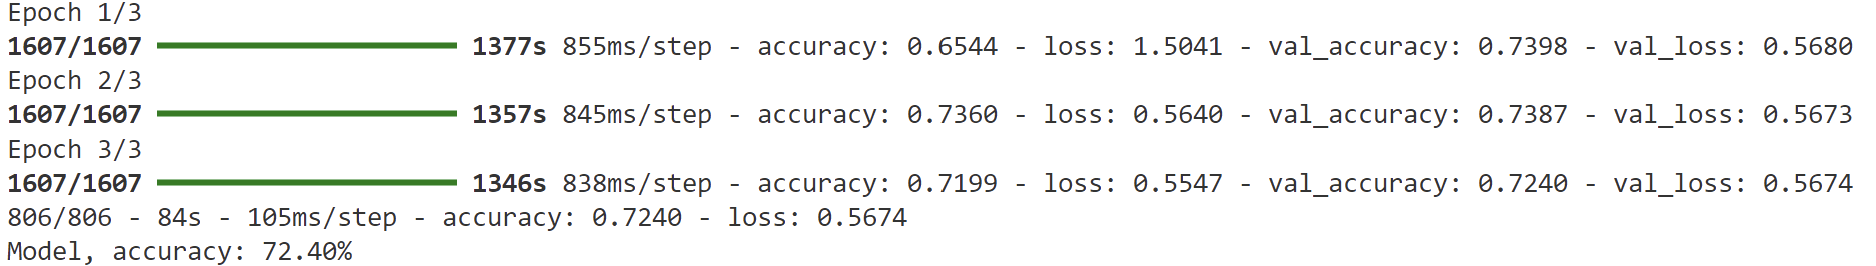
\includegraphics[width=1\linewidth]{Screenshot 2024-05-25 231244.png}
    \caption{Epoch Training and Model Accuracy}
    \label{fig:enter-label}
\end{figure}
Ultimately, the training process takes almost 2 hours. The loss function we used is the binary cross-entropy loss function:
\[Loss = -\frac{1}{N} \sum_{n=1}^{N} y_i \cdot log(p(y_i))+(1-y_i) \cdot log(1-p(y_i))\]
This sums over the log of the probabilities of a given outcome multiplied by that outcome and averages over it. We use this loss function because each output label is determined independently of the others. \\

Using this model resulted in a test performance of 72.40\%. Although this is not a seemingly high result, given the problem complexity, we believe it is adequate. One caveat to this is that nearly all of the games had at least one tag in common, so predicting that tag was nearly guaranteed with our model. Furthermore, we can use keras' \verb|predict()| function, which outputs the probability of a given observation belonging to one of the labels. \\

Below is an example output of the actual targets for a set of 5 images:
\begin{verbatim}
        [[1 0 1 0 1 0 1 1 0 0 0 1 0 0 1 0 1 1 0 1]
         [1 0 1 0 1 0 1 1 0 0 0 1 0 0 1 0 1 1 0 1]
         [1 0 1 0 1 0 1 1 0 0 0 1 0 0 1 0 1 1 0 1]
         [1 0 1 0 1 0 1 1 0 0 0 1 0 0 1 0 1 1 0 1]
         [1 0 1 0 1 0 1 1 0 0 0 1 0 0 1 0 1 1 0 1]]
\end{verbatim}
And the (rounded) predicted targets produced by the model:
\begin{verbatim}
        [[1 0 0 0 0 0 0 0 0 0 0 0 0 0 0 0 0 0 0 0]
         [1 0 0 0 0 0 0 0 0 0 0 0 0 0 0 0 0 0 0 0]
         [1 0 0 0 0 0 1 0 0 0 0 0 0 0 0 0 0 0 0 0]
         [1 0 1 0 0 0 1 0 0 0 0 0 0 0 0 0 1 0 0 0]
         [1 0 0 0 0 0 0 0 0 0 0 0 0 0 0 0 0 0 0 0]]
\end{verbatim}

Because this is a multilabel classification problem, each observation outputs a vector of probabilities. We used the \verb|np.round()| function to round each probability to the nearest whole number (which is a threshold of >0.5). Upon manual review, we found that the model is far more likely to output \textbf{false negatives} than false positive, that is, a score of 0 when it should be 1 is more likely than a score of 1 that should be 0. In some cases, the model only predicted the existence of the most frequently occurring tag, and none of the other tags that were there on the actual labels. This indicates that some labels were much harder for the model to train for, which may be due to these labels infrequently occurring in both the training set and test set. \\



For future exploration, it might be interesting to explore only the top 5 or 10 tags, as it appears to be that only a few tags are frequently occurring in the dataset. It is clear after constructing the model for the top 20 tags that there is not enough information for the model to be trained on this many tags, which is likely causing the false negatives.

\section{Text Streaming}
In the third assignment, we use Spark with the notebook provided on our laptop. Data to be collected is the text from Hacker News listed by time with the most recent one on top. It will be put to frontpage by an internal algorithm, which we want to predict by our model if it will happen in 6 hours (label). We suggest logistic regression approach as the standard model, which is available in scikit-learn. In case of the frequency of the gained points, the feature can be key words.\\
However, Spark is working correctly with park$\_$example.ipynb with the notebooks provided, and data can also be saved in the documents, but the streaming, which only has .crc file rather than JSON file, suggest we are not correctly collecting the data. Moreover, to process it we find it might be more proper to use spark.ml (MLlib). 

\section{Network Analysis}
For this assignment, we utilized memgraph's community detection query module, \verb|community_detection.get()|. Memgraph's community detection algorithm uses the Louvain method, which runs in O(nlogn) complexity time, making it suitable for our relatively large dataset with over 1 million relationships and over 300 thousand nodes. \\

We first implemented the following query which added an attribute to each node with their respective communities:
\begin{verbatim}
    CALL community_detection.get()
    YIELD node, community_id
    SET node.community_id = community_id;
\end{verbatim}
Then, the following query was used to return the first 1000 relationships:
\begin{verbatim}
    MATCH (u:User)-[e]-(t:Tweet)
    RETURN * LIMIT 1000;
\end{verbatim}
We also ran this query with a limit of 5000 for a more complex visualization. In addition to these queries, we also utilized python to determine the percentage of each language within a community, to see if there was any overlap, and to verify in an additional way apart from visually the connection between communities and language. 

We found that among the first 1000 relationships, one individual account became a focal point for online interaction. Additionally, when we increase the relationships to the first 5000, we see that multiple focal points exist, each becoming a centerpoint for their respective communities. 
If we look closer at each center, it is clear that language plays a strong role in determining the communities. Most tweet nodes, and by extension user nodes, share a common language in a community. Note that there are some errors in the initial data input, as some languages are listed as qmc or otherwise, when they are likely to be more fitting with their surrounding nodes. To project the networks, all visualizations utilized Gephi's force atlas layout tool. Additional modifications were made to allow for ease of understandability of distinctive communities, such as coloring. 
\begin{figure}[h!]
    \centering
    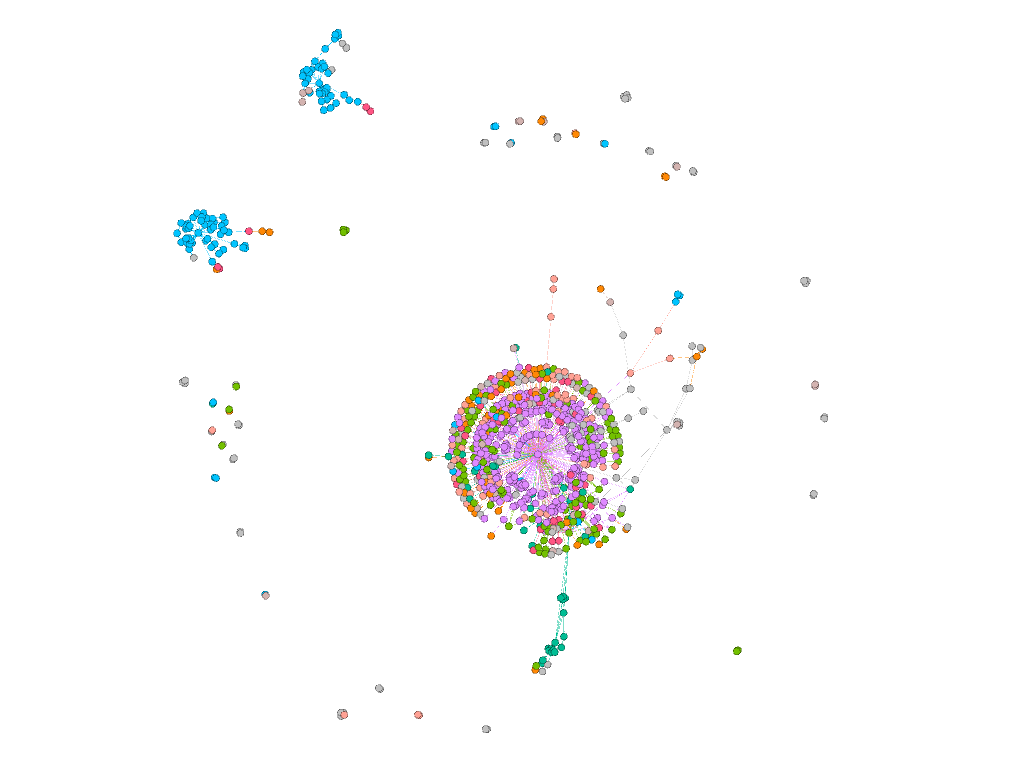
\includegraphics[width=0.8\linewidth]{Graph Analytics/graph_1k.png}
    \caption{1000 User-Tweet Relationships Visualized}
    \label{fig:enter-label}
\end{figure} 
\begin{figure}[h!]
\centering
\begin{subfigure}{.6\textwidth}
  \centering
  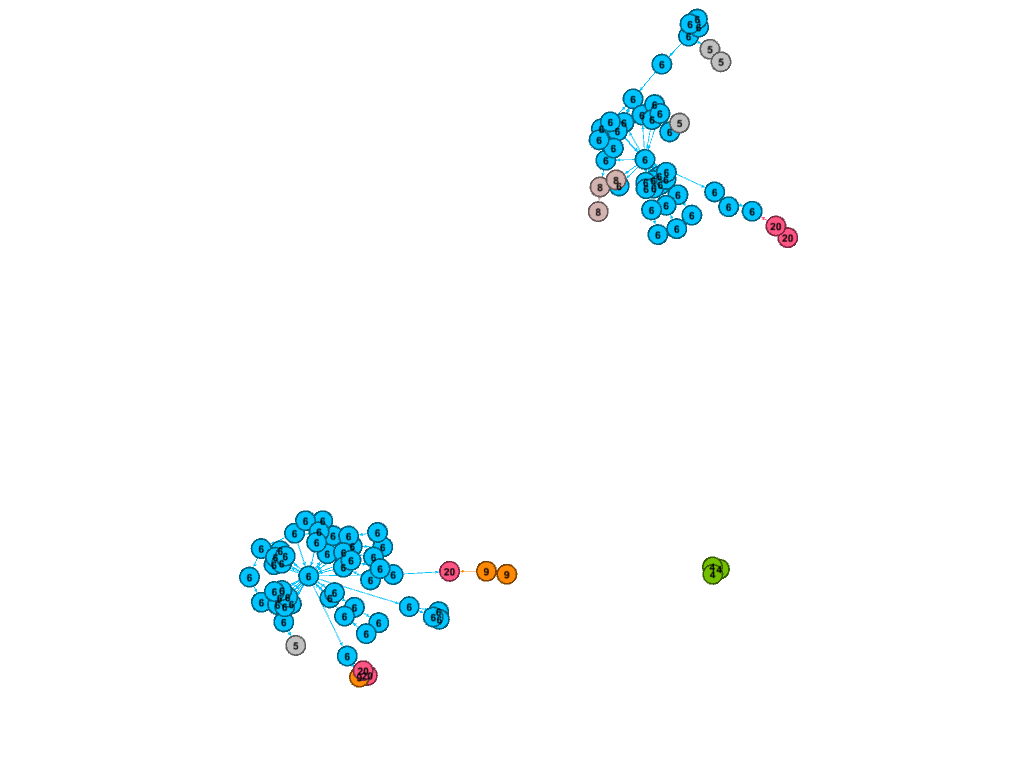
\includegraphics[width=.6\linewidth]{Graph Analytics/graph_1k_com6.png}
  \caption{Community 6 (blue nodes) }
  \label{fig:sub1}
\end{subfigure}%
\begin{subfigure}{.6\textwidth}
  \centering
  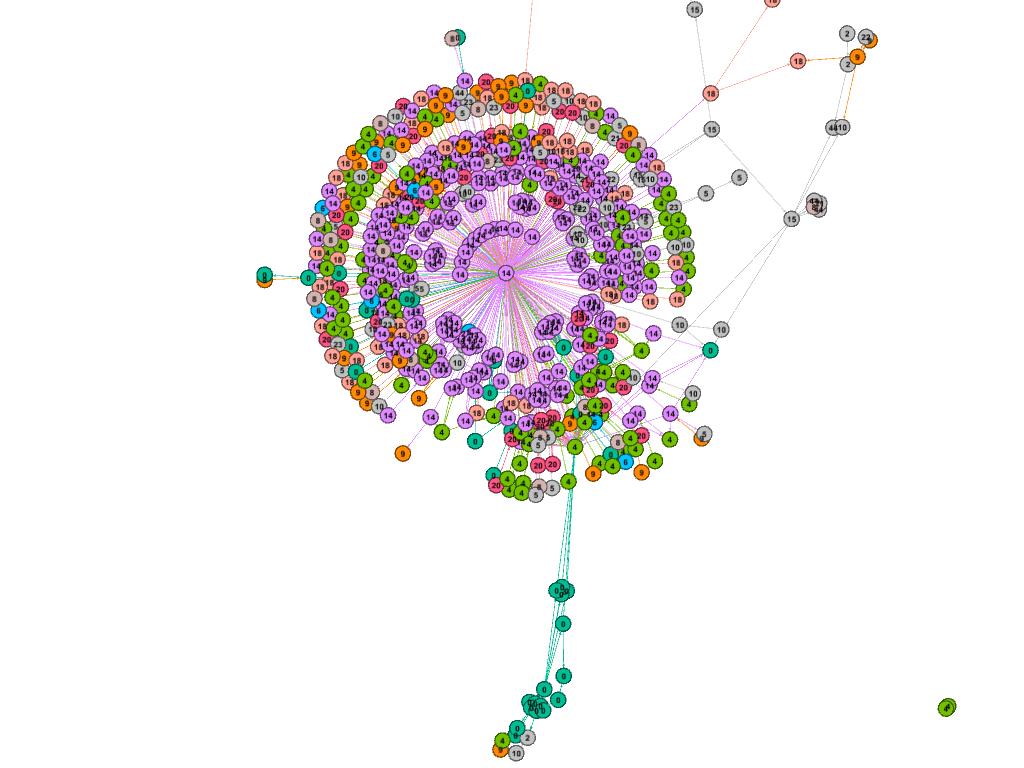
\includegraphics[width=.6\linewidth]{Graph Analytics/graph_1k_com14.png}
  \caption{Community 14 and 4 (purple and green nodes)}
  \label{fig:sub2}
\end{subfigure}
\caption{Communities in First 1000 User-Tweet Relationships}
\label{fig:test}
\end{figure}

Figures (a) and (b) focus on communities 6 and 14 respectively within the first 1000 relationships. These were the most unique communities to be seen, however in subfigure (b) we can see that there is more variation, which is due to the strong presence of community 4 intertwined. In fact, the top 3 most frequent communities within the first 1000 relationships were 14, 4, and 6, in that order. Over 30\% of the nodes belonged to community 14, and slightly more than 12\% of the nodes belonged to communities 4 and 6 each. \\

We also sought to visualize 5000 relationships, to see if there would be any interesting development in terms of communities:
\begin{figure}[h!]
    \centering
    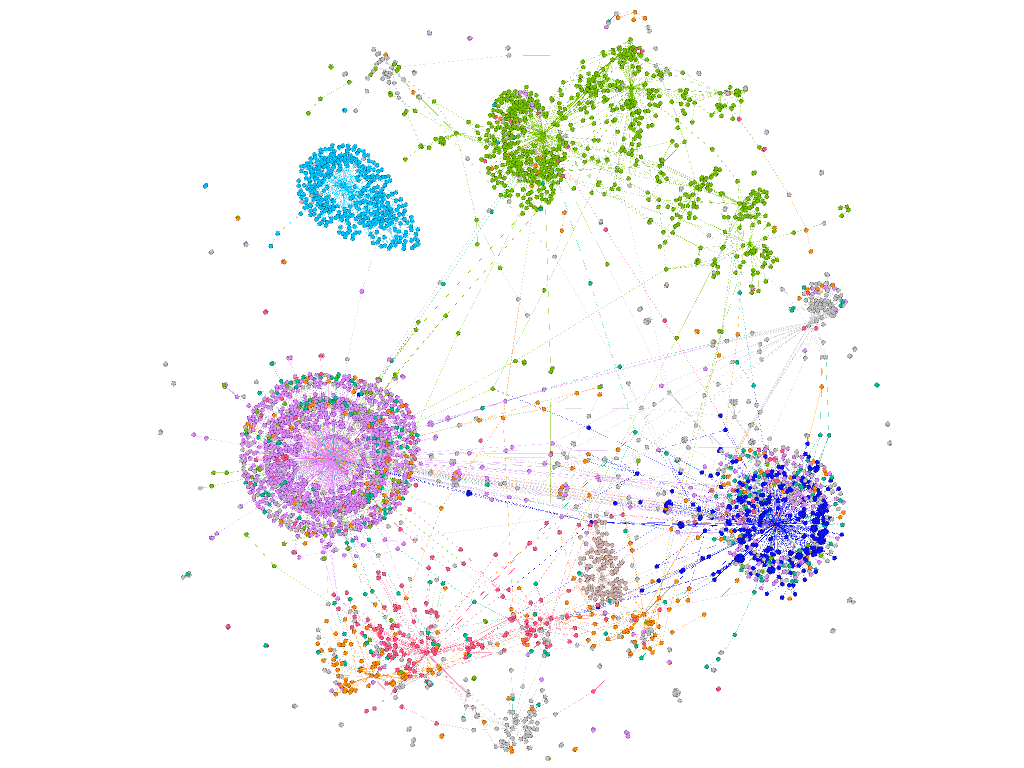
\includegraphics[width=0.8\linewidth]{Graph Analytics/5kwide.png}
    \caption{5000 User-Tweet Relationships Visualized}
    \label{fig:enter-label}
\end{figure} 
\begin{figure}[h!]
\centering
\begin{subfigure}{.6\textwidth}
  \centering
  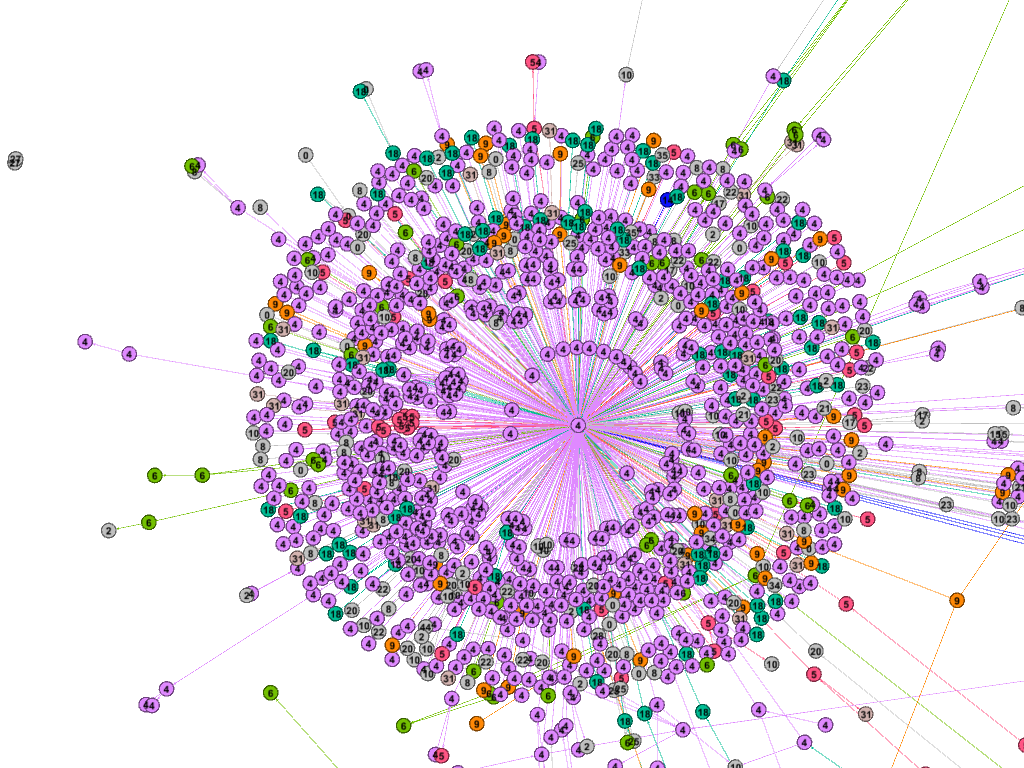
\includegraphics[width=.6\linewidth]{Graph Analytics/5k_com4.png}
  \caption{Community 4}
  \label{fig:sub1}
\end{subfigure}%
\begin{subfigure}{.6\textwidth}
  \centering
  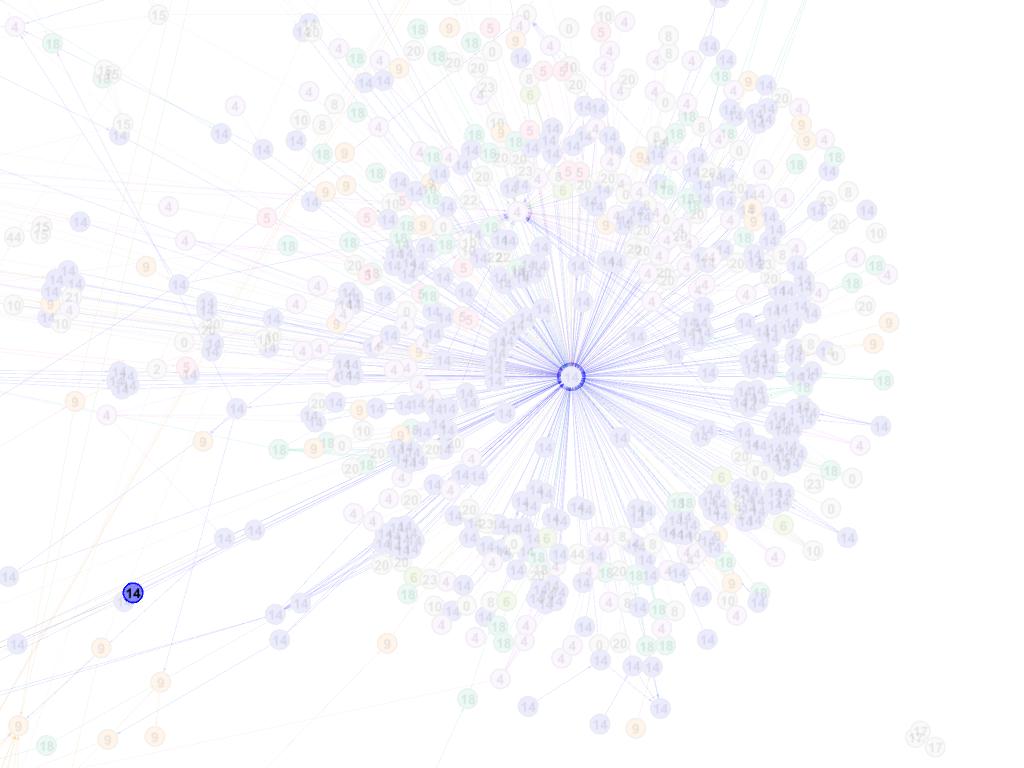
\includegraphics[width=.6\linewidth]{Graph Analytics/5k_com14.png}
  \caption{Community 14}
  \label{fig:sub2}
\end{subfigure}
%\caption{Communities in First 5000 User-Tweet Relationships}
\label{fig:test}
\begin{subfigure}{.6\textwidth}
  \centering
  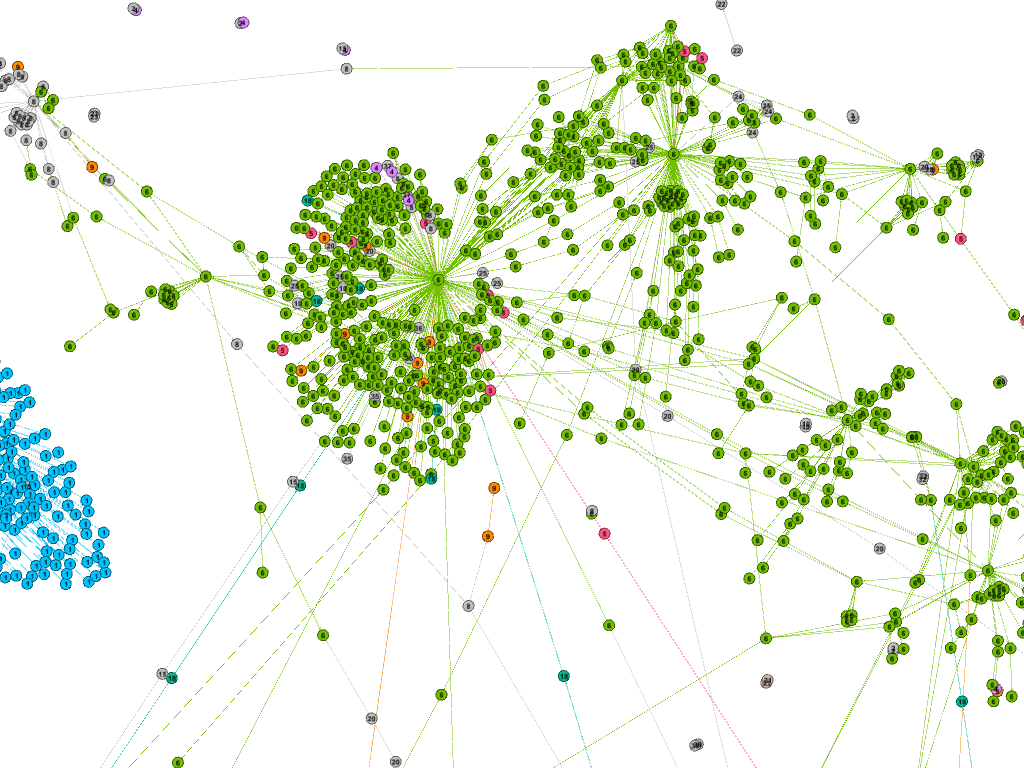
\includegraphics[width=.6\linewidth]{Graph Analytics/5k_com_others.png}
  \caption{Other communities formed in 5000 User-Tweet Relationships}
  \label{fig:sub2}
\end{subfigure}
\caption{Communities in First 5000 User-Tweet Relationships}
\label{fig:test}
\end{figure}
With 5000 relationships visualized in a network graph, we see that the most present community is 14. Additionally, we can see that communities have become relatively more defined, with fewer overlaps than compared with just 1000 relationships visualized. Additionally, we can see that although the nodes belonging to community 6 (green nodes) are more sparsely located, there are still very few nodes from other communities in their proximity. Comparatively, communities 14 and 4 from 1000 relationships had significant overlap location-wise. \\

\subsection{Community-Language Relationship}
Though we have explored how the nodes can be visually separated by communities (obtained from the Louvain algorithm), we have yet to explore the relationship between community and the languages used. In this section, we explore that relationship and demonstrate a fairly strong correlation between community membership and language.\\

One caveat that should be mentioned prior to further exploration is that some nodes are not properly labeled with the \verb|lang| property. For instance, qme and zxx are sometimes listed as the tweet language, however these do not represent any language (as far as we can tell). It is also possible that they are Dutch or French language tweets mistakenly attributed to this label. If true, this would in fact substantiate the findings below even further. \\

The top 10 communities in terms of node membership all predominantly used the languages of French (fr), Dutch (nl), or English (en) for tweeting (X-ing?). Community 6 had over 75\% of its member nodes utilize French, and was the most frequent community in terms of membership. The second most frequent community was community 25, also a predominantly French-using community, where 85\% of tweets were written in this language. Interestingly, these were the only French speaking communities in the top 10, as the rest were either Dutch-speaking or English-speaking communities. The next most common communities were 4, 18, and 9, all of which utilize Dutch as the primary language of choice, by significant margins. To further cement our findings of a relationship between language and community membership, we conducted a Chi-squared test, which proved a significant relationship. The test statistic equalled 1200513.077, and the p-value was well below the 0.05 threshold. The code for this test was written in python, and is listed in the appendix. Thus, we can clearly state that there is a strong relationship between language used and community membership.\\

For further analysis, one could also approach the connection between political affiliation and communities, particularly within the frame of context of how languages affected communities. It is clear that communities could be divided very cleanly between languages, but that some languages like French and Dutch had multiple communities. Then, one could pose the question has to how these communities, within the context of language, were formed. \



















\newpage


\section{Appendix}

The program code for all assignments can be found in the linked github repository: \url{https://github.com/theokristoffer/Advanced-Analytics-Code}.
\\\href{https://github.com/theokristoffer/Advanced-Analytics-Code}
\\

There are additional programs that allowed for further insight for some of the assignments, and files that allowed for analysis.
Note that the \verb|community_mining.json| file used in the chi-squared analysis was too large to be appended to the repository, as it contained all information on relationships between users and tweets from the fourth assignment. Below is the entire program used for the multilabel image classification. The github repository also contains the full program for all analyses completed in the first assignment. \\

\textbf{Programs for first assignment:} 
\begin{itemize}
    \item \verb|assignment1.py|
\end{itemize}


\textbf{Programs for second assignment:}
\begin{itemize}
    \item \verb|resize.py|
    \item \verb|game_rec_modified.py|
    \item \verb|y_test.csv|
    \item \verb|binary_predictions.csv|
\end{itemize}

\textbf{Programs and files for fourth assignment:} 
\begin{itemize}
    \item \verb|independence test.py|
    \item \verb|ratios_csv.csv|
    \item \verb|5k_graph.graphml|
    \item \verb|memgraph_1k.graphml|
\end{itemize}




\end{document}
